\chapter{Evaluation and Discussion}
\label{chap:eval}

\section{Navigation}

In this chapter, we present the results of our work. In Section~\ref{sec:purpose_of_evaluation} we discuss the goals of the evaluation, in Section~\ref{sec:eval_procedure} we describe how we performed the evaluation of results, then in Section we describe practical implications of our project, then Limitation, then summary of the chapter.



\section{Purpose of the evaluation}
\label{sec:purpose_of_evaluation}
The evaluation aimed to achieve two interconnected objectives:
    \begin{enumerate}
        \item Automation of Responses: To ensure the system can autonomously generate and deliver answers to user inquiries without manual intervention.
        
        \item Quality Assurance: To guarantee that these automated answers align with Hanafi fiqh principles and NamazApp’s functional requirements, ensuring accuracy and reliability.
    \end{enumerate}
The system’s success depends on balancing these goals: avoiding the risks of automating incorrect answers (which could mislead users) and failing to automate correct answers (which reduces efficiency). To measure this balance, we defined four evaluation categories:

    \begin{enumerate}
        \item True positive(TP) -- Correct answer sent to the user.
        \item True negative(TN) -- Incorrect answer withheld.
        \item False positive(FP) -- Incorrect answer sent to the user.
        \item False negative(FN) -- Correct answer withheld.
    \end{enumerate}
This framework allowed us to identify gaps in both the automation process (e.g. overly cautious decision-making) and answer quality (e.g. errors in religious guidance).
\section{The evaluation procedure}
\label{sec:eval_procedure}

As we said earlier, we implemented three versions of the pipeline. Firstly, we ran the v1 pipeline on the real user data (pending active conversations). We processed 98 units. Then we took these conversations as dataset and ran the v2 and v3 pipeline on them. This allowed us to compare the results of different pipeline versions.

\subsection{Stage 1: Real-User Testing}

    \begin{itemize}
        \item Data: We used 98 real active conversations with NamazApp users.
        \item Process: The system generated answers and decided whether to send them. These results went to a Telegram group for review.
        \item Review Steps:
            \begin{enumerate}
                \item Our team checked if answers were religiously correct and useful for the app.
                \item We also checked if the system’s choice to send/not send made sense.
            \end{enumerate}
        \item Iterative refinement: As issues were found, we updated the system’s knowledge base to fix gaps or errors.
    \end{itemize}

\subsection{Stage 2: Refining the system based on the Results - creating v2}

After analyzing the results of the first pipeline version, we realized that the question extraction is one of the weakest points - many false positives appeared because of the incorrect question extraction. That is why we created the second version of the pipeline with improved prompt for question extraction.

    \begin{itemize}
        \item Data: We used the same 98 real active conversations with NamazApp users.
        \item Process: We collected these conversations in a csv table and run the pipeline v2 on them
        \item Review Steps:
            \begin{enumerate}
                \item Check the correctness of the answers
                \item Check the send decision
                \item Compare the results with the previous version
            \end{enumerate}
        \item We decided to create a version 3 that integrates IslamQA knowledge base.
    \end{itemize}

\subsection{Stage 3: Adding IslamQA knowledge base integration - creating v3}

Version 2 of the pipeline has successfully improved the question extraction, and therefore, the results. The next step is to integrate the IslamQA database to increase the amount of correct answers.

% \section{Collected data and evaluation results}

% This section describes how we collected the data, how we annotated it, and what results we got.

% \subsection{Data collection}

% The NamazApp mobile application has a specific Q\&A section, where users can ask anything. All pending conversations are recorded in the database and marked active. Here by active conversations, we mean the conversations that have unanswered messages. For the evaluation stage, we took 98 unique active conversations from the database. These conversations might contain questions; moreover, some can already be answered. The questions objective can be divided into several topics: questions about the app (e.g. how to use some functionality), general questions about Islam (e.g. how to pray), and personal questions with specific context. In Table X.X the topic distribution is presented.

\section{Evaluation results}
\label{sec:evaluation_results}

This section describes the evaluation results of three pipeline versions.
% Next, we executed the system's RAG pipeline. It processed each user's active conversation, extracted questions from it, retrieved similar PAQs, generated the answer, and decided whether the answer should be sent to the user. The pipeline response included both the answer and the decision to send. The answer is generated, even if it is not sent. The correctness of the answers intended for sending was manually annotated by a reviewer. The reviewer was the lead of the NamazApp project. He has deep knowledge of how the app works; moreover, he has basic Islamic Fiqh knowledge, so he is eligible to answer the questions from the app users, who are beginners in practicing religion. 

In Tables \ref{tab:correctness_dispatch_cm_v1}, \ref{tab:correctness_dispatch_cm_v2}, \ref{tab:correctness_dispatch_cm_v3} we present the confusion matrices for three pipeline versions respectively based on the answer's correctness and the send decision. In Fig.~\ref{fig:confusion-chart} the comparison between three versions is presented based on these four categories, and in Fig.~\ref{fig:metrics-chart} derived metrics, such as presicion, recall and F1-score are compared between the versions of the pipeline. As we can see, Precision (TP / (TP + FP)) increased from 70\% in v1 to 82,53\% v3, indicating the number of correct answers that were sent out of the total sent answers, Recall (TP / (TP + FN)), that represents how many correct answers were sent, eventually is 69\%. The F1-score (2 * (Precision * Recall) / (Precision + Recall)) that takes into account both Precision and Recall is 75\% in v3 version.

\makeatletter
\let\@currsize\normalsize
\makeatother

\begin{longtable}{l|cc|c}

\caption[Confusion Matrix V1: Answer Correctness and Send Decision]{
    Confusion Matrix V1: Answer Correctness and Send Decision
} \label{tab:correctness_dispatch_cm_v1} \\

\toprule
\multicolumn{1}{c}{} & \multicolumn{2}{c}{\textbf{System Action}} & \multicolumn{1}{c}{} \\*
\cmidrule(lr){2-3}
\textbf{Actual State} & \textbf{Sent Answer} & \textbf{Did Not Send Answer} & \textbf{Total Actual} \\*
\midrule
\endfirsthead

\textbf{Answer Correct} & \textbf{TP} & \textbf{FN} & \\
                      & \textit{(Correctly Sent)} & \textit{(Correctly Not Sent)} & 71 \\
                      & 47 & 24 & \\*
\midrule

\textbf{Answer Wrong} & \textbf{FP} & \textbf{TN} & \\
                     & \textit{(Wrongly Sent)} & \textit{(Wrongly Not Sent)} & 27 \\
                     & 20 & 7 & \\*
\midrule

\textbf{Total Actions} & 67 & 31 & 98 \\
                       & (TP + FP) & (FN + TN) & \\

\end{longtable}

\makeatletter
\let\@currsize\normalsize
\makeatother

\begin{longtable}{l|cc|c}

\caption[Confusion Matrix V2: Answer Correctness and Send Decision]{
    Confusion Matrix V2: Answer Correctness and Send Decision
} \label{tab:correctness_dispatch_cm_v2} \\

\toprule
\multicolumn{1}{c}{} & \multicolumn{2}{c}{\textbf{System Action}} & \multicolumn{1}{c}{} \\*
\cmidrule(lr){2-3}
\textbf{Actual State} & \textbf{Sent Answer} & \textbf{Did Not Send Answer} & \textbf{Total Actual} \\*
\midrule
\endfirsthead

\textbf{Answer Correct} & \textbf{TP} & \textbf{FN} & \\
                      & \textit{(Correctly Sent)} & \textit{(Correctly Not Sent)} & 70 \\
                      & 52 & 18 & \\*
\midrule

\textbf{Answer Wrong} & \textbf{FP} & \textbf{TN} & \\
                     & \textit{(Wrongly Sent)} & \textit{(Wrongly Not Sent)} & 28 \\
                     & 12 & 16 & \\*
\midrule

\textbf{Total Actions} & 64 & 34 & 98 \\
                       & (TP + FP) & (FN + TN) & \\

\end{longtable}

\makeatletter
\let\@currsize\normalsize
\makeatother

\begin{longtable}{l|cc|c}

\caption[Confusion Matrix V3: Answer Correctness and Send Decision]{
    Confusion Matrix V3: Answer Correctness and Send Decision
} \label{tab:correctness_dispatch_cm_v3} \\

\toprule
\multicolumn{1}{c}{} & \multicolumn{2}{c}{\textbf{System Action}} & \multicolumn{1}{c}{} \\*
\cmidrule(lr){2-3}
\textbf{Actual State} & \textbf{Sent Answer} & \textbf{Did Not Send Answer} & \textbf{Total Actual} \\*
\midrule
\endfirsthead

\textbf{Answer Correct} & \textbf{TP} & \textbf{FN} & \\
                      & \textit{(Correctly Sent)} & \textit{(Correctly Not Sent)} & 75 \\
                      & 52 & 23 & \\*
\midrule

\textbf{Answer Wrong} & \textbf{FP} & \textbf{TN} & \\
                     & \textit{(Wrongly Sent)} & \textit{(Wrongly Not Sent)} & 23 \\
                     & 11 & 12 & \\*
\midrule

\textbf{Total Actions} & 63 & 35 & 98 \\
                       & (TP + FP) & (FN + TN) & \\

\end{longtable}

\begin{figure}
    \centering
    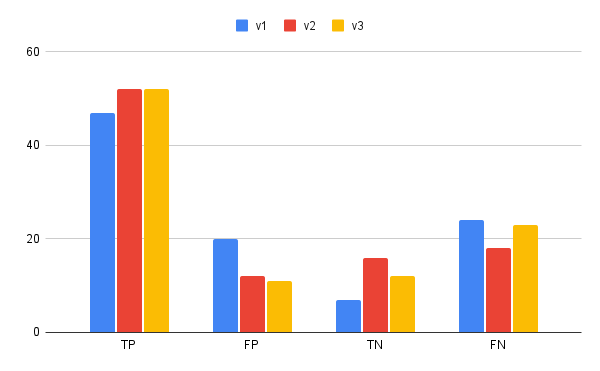
\includegraphics[width=1\linewidth]{figs/confusion_chart.png}
    \caption{Bar chart with confusion matrix results of three pipeline versions}
    \label{fig:confusion-chart}
\end{figure}

\begin{figure}
    \centering
    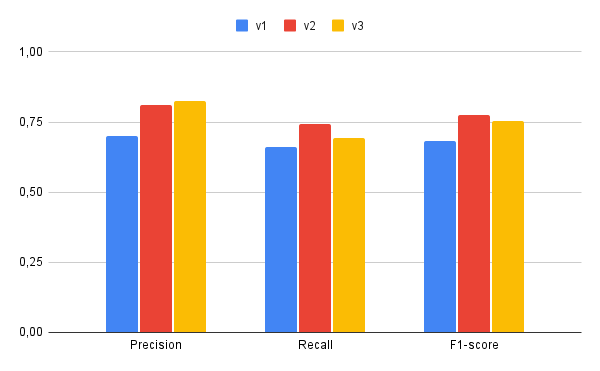
\includegraphics[width=1\linewidth]{figs/metrics_chart.png}
    \caption{Bar chart with result metrics of three pipeline versions}
    \label{fig:metrics-chart}
\end{figure}

\subsection{Key findings}

The evaluation results show us that the system works with high precision, especially when dealing with questions that have relevant PAQs. Also, the improvements of the second and third versions increased the precision, which is the main goal.

In Section \ref{sec:evaluation_results} we described the metrics calculated based on the results we obtained: Precision, Recall, and F1-Score. These metrics are especially significant for us. First, high precision is important because it shows the system has high reliability: sending wrong answers is minimized. It is crucial in such high-stakes situations when an incorrect answer could lead to a negative outcome. Second, the recall has a lower value, which means that not all the correct answers were indeed sent. This metric is not so important as precision. However, the high recall indicates that the system is beneficial in achieving our main goal - automating the answering questions and making it more efficient. We can observe that the v2 enhancement increased recall, but v3 decreased it. This result is expected, since v3 integrates the IslamQA database - so the number of false negatives increased because only the answers that are based on PAQs are sent to the user. Third, the F1-score shows us the overall picture of the results.  

True negatives are mostly occurring in cases where the LLM generated the answer with the absence of relevant PAQs. This is a desired behavior since high reliability is more important than high recall.
False positives occurred because of several reasons. One of the most frequent in the v1 was the incorrect extraction of the questions from a conversation. That is why we introduced the v2. Moreover, the relatively small size of the PAQs database when the retrieved PAQs are not significantly relevant semantically. This is a key point of the system improvement, since it directly affects the precision.

As we discussed earlier, the presence of relevant PAQs strongly affects the result. Therefore, the PAQ database is the main limitation of the system. Our PAQ database has a limited amount of questions, and they are dedicated to a narrow topic.

\subsection{Practical implications}

The system is successfully integrated with the NamazApp project, improving the user experience by lowering the reply time: the users get answers to frequently asked questions immediately. Moreover, the workload of human experts became significantly less: now they are not answering simple questions, instead, they review the system's answers and focus on challenging questions. Furthermore, this system has the potential to become a separate project, expanding the scope of the application.

\subsection{Future work}

One of the areas of future work might be applying advanced RAG techniques such as modular RAG. Moreover, the comparison of different approaches, such as pretraining, advanced RAG, and prompt engineering techniques, could be performed. Moreover, the ability to clarify questions might lead to better results. Furthermore, the exploring of how to overcome the database limitation is also important.

\subsection{Conclusion}

This chapter observed and compared the evaluation results of the three pipeline versions. We revealed the key limitations, of each version, and iteratively improved our solution. Moreover, we addressed the limitations of the final version and proposed a work for future studies.


% \section{Contradicting results}
% \section{Unexpected findings}
% \section{Comparison with previous studies}
% \section{Practical implications and Future research}
% \section{Limitations}

% \section{Summary}